\documentclass[10pt,aspectratio=43]{beamer}
\usepackage{fsu2017}
% the aspactratio defines the foramt
% default is 43 (4:3, 128mm:96mm), alternatives are
% 32 (3:2, 135mm:90mm)
% 54 (5:4, 125mm:100mm)
% 149 (14:9, 14cm:9cm)
% 169 (16:9, 16cm:9cm)
% 1610 (16:10, 16cm:10cm)
% 141 (1.41:1, 148.5mm:105mm, ratio of DinA)

\usepackage{color}
\usepackage[backend=biber,style=authoryear]{biblatex} % or any other style you prefer
\addbibresource{references.bib}


% graphic settings
\usepackage{graphicx}
\usepackage{tikz}
\usepackage{pgfplots}
\usepackage{amsmath}
\usepackage{accents}
\usepackage{booktabs}
%\usepackage{appendixnumberbeamer}
\usetikzlibrary{arrows.meta, positioning, calc}
\pgfplotsset{compat=1.18}
\newcommand{\myvect}[1]{\accentset{\rightharpoonup}{#1}}

\usetikzlibrary{angles, quotes, shapes, decorations.markings, calc, arrows.meta,3d, shapes.multipart}
% Styles
%% Node Style in Order Text to Get Center Alignment
\tikzset{every text node part/.style={align=center}}
%% Bottom Ray Outside Box
\tikzset{
	every text node part/.style = {align=center},
	rayE2/.style = {
		postaction = decorate,
		decoration = {
			markings,
			mark = at position 0.52 with {\arrow{stealth}}
		}
	}
}

% Custom citation: author + title only
\DeclareCiteCommand{\authortitlefootcite}
{\usebibmacro{prenote}}
{%
	\printnames{labelname}%
	\addcomma\space%
	\printfield[citetitle]{title}%
	\addcomma\space
	\printdate% year (from date/year field)
}
{\multicitedelim}
{\usebibmacro{postnote}}

\newcommand{\backupbegin}{
	\newcounter{framenumberbeforeappendix}
	\setcounter{framenumberbeforeappendix}{\value{framenumber}}
}
\newcommand{\backupend}{
	\addtocounter{framenumber}{-\value{framenumberbeforeappendix}}
}



\title[Parameter estimation with correlated photon pairs]{Parameter estimation\\with correlated photon pairs}
\author[Jan Gößwein]{Jan Gößwein}
\date{Jena, \today}
\institute[IAP]{Institute of Applied Physics}

\begin{document}
	
	%% titlepage
	\showheadlinefalse
	\begin{frame}[noframenumbering]
		\titlepage
	\end{frame}
	
	
	
	
%	\showheadlinefalse
%	\begin{frame}{Table of content}
%		\tableofcontents
%	\end{frame}
	
	\showheadlinetrue
	
	\section{Motivation}
	
	\begin{frame}{Motivation}
		\begin{center}
			
			
			\begin{tikzpicture}[baseline, node distance=1cm and 2cm]
				
				% Top image
				%			\visible<2->{\node (p)  {\includegraphics[width=.35\textwidth]{Images/ConvImage}};
					%				
					%			}
				%			\visible<3->{
					%				\node (a) [below=of p] {\includegraphics[width=.35\textwidth]{Images/CoincImage}};
					%				\draw[-{Latex[length=2mm]}, thick] (p.west) to[bend right=20] node[right] {correlations \only<3->{%
							%						\footnote{\authortitlefootcite{bridaExperimentalRealizationSubshotnoise2010}
								%					}}} (a.west);
					%				
					%			}
				
				% Bottom image
				
				\visible<2->{
					\node (b) %[right=of p]
					{\includegraphics[width=.35\textwidth]{Images/ConvImageNoise}};
					% Arrows
					
					%\draw[-{Latex[length=2mm]}, thick] (p.east) to node[above] {add noise} (b.west);
				}
				%\coordinate (mid) at ($ (p)!0.5!(b) $);
				\visible<3->{
					\node (c) [below=of b] {\includegraphics[width=.35\textwidth]{Images/CoincImageNoise}};
					% Arrows
					
					\draw[-{Latex[length=2mm]}, thick] (b.east) to[bend left=30] node[right] {correlations \only<3->{	\footnote{\authortitlefootcite{bridaExperimentalRealizationSubshotnoise2010}
					}}} (c.east);
				}
			\end{tikzpicture}
		\end{center}
		\vspace*{2em}
		\visible<4->{
			\textbf{Objective:} Can correlated photons provide advantages in terms of precision in noisy regimes for parameter estimation?
		}
		
	\end{frame}
		
%	\begin{frame}{Motivation}
%			% Start a TikZ picture environment
%			\begin{center}
%				
%			
%			\begin{tikzpicture}[baseline, node distance=2cm and 2cm]
%				
%				% Top image
%				\visible<2->{\node (p)  {\includegraphics[width=.15\textwidth]{Images/PureImage.pdf}};
%				
%				}
%				\visible<3->{
%				\node (a) [right=of p] {\includegraphics[width=.15\textwidth]{Images/NoisyImage.pdf}};
%				\draw[-{Latex[length=2mm]}, thick] (p.east) -- node[above] {add noise} (a.west);
%				
%				}
%				
%				% Bottom image
%				
%				\visible<4->{
%				\node (b) [right=of a] {\includegraphics[width=.15\textwidth]{Images/BetterImage.pdf}};
%				% Arrows
%				
%				\draw[-{Latex[length=2mm]}, thick] (a.east) to node[above] {correlations \footnote<4->{\authortitlefootcite{bridaExperimentalRealizationSubshotnoise2010}}} (b.west);
%				}
%			\end{tikzpicture}
%			\end{center}
%			\vspace*{3em}
%			\visible<5->{
%			\textbf{Objective:} Can correlated photons provide advantages in terms of precision in noisy regimes for sensing?
%			}
%	\end{frame}
	
	\section{Theory}
	
	\begin{frame}{Spontaneous parametric \\down-conversion}
		\visible<2->{
			\begin{minipage}{.4\textwidth}
				\begin{center}
					\resizebox{.7\textwidth}{!}{%
						\includegraphics[scale=1]{Images/SPDC_Cone.pdf}
					}%
				\end{center}
			\end{minipage}
		}
		%			\begin{minipage}{.45\textwidth}
			%			\begin{center}
				%				\resizebox{\textwidth}{!}{%
					%					\begin{tikzpicture}
						%						%\useasboundingbox (0,0) rectangle (10,14);
						%						\tikzstyle{every node}=[font=\LARGE]
						%						
						%						\draw [line width=2.5pt, rayE2,color=blue] (2.5,15.25) -- (6.25,15.25);
						%						\draw [line width=2.5pt, rayE2,color=black!40!green] (8.5,15.25) -- (12,16.75);
						%						\draw [line width=2.5pt, rayE2,color=red] (8.5,15.25) -- (12,13.75);
						%						\draw [ fill=black!10 , line width=1.6pt , rounded corners = 9.0] (6.25,16) rectangle (8.5,14.5);
						%						
						%						\node at (7.45,15.25) {$\chi^2$};
						%						\node at (4.4,15.75) [color=blue] { $\lambda_{\text{p}}$};
						%						\node at (10.3,16.8) [color=black!40!green] { $\lambda_{\text{s}}$};
						%						\node at (10.3,13.7) [color=red] { $\lambda_{\text{i}}$};
						%					\end{tikzpicture}
					%				}%
				%			\end{center}
			%			\end{minipage}
		\hfill
		\begin{minipage}{.5\textwidth}
			\visible<3->{
				\centering
				\resizebox{\textwidth}{!}{%
					\begin{tikzpicture}
						\begin{axis}[
							ymin=0,
							ymax=650,
							xmin=-16,
							xmax=16,
							xlabel={Time Delay [ns]},
							ylabel={Coincidence counts [a.u.]},
							xtick={-15,-10,-5,0,5,10,15},
							bar width=2,
							minor y tick num = 3,
							area style,
							width=10cm,
							height=7cm,
							every axis plot/.append style={fill=gray!40},
							legend style={at={(0.5,1.05)}, anchor=south, legend columns=-1},
							legend cell align=left
							]
							
							% --- Shaded middle region: Coincidences ---
							\only<4->{
								\addplot [
								fill=green,
								fill opacity=0.3,
								draw=none
								] coordinates {
									(-2,650)
									(2,650)
									(2,0)
									(-2,0)
								};
								\addlegendentry{Coincidences}
								
								% --- Vertical dashed lines ---
								\draw[dashed, thick] (axis cs:-2,0) -- (axis cs:-2,650);
								\draw[dashed, thick] (axis cs:2,0) -- (axis cs:2,650);
								
							}
							
							% --- Shaded left region: Accidentals ---
							
							\only<5->{
								\addplot [
								fill=red,
								fill opacity=0.3,
								draw=none
								] coordinates {
									(-16,650)
									(-2,650)
									(-2,0)
									(-16,0)
								};
								\addlegendentry{Accidentals}
								
								
								% --- Shaded right region: Accidentals ---
								\addplot [
								fill=red,
								fill opacity=0.3,
								draw=none
								] coordinates {
									(2,650)
									(16,650)
									(16,0)
									(2,0)
								};
							}
							
							
							% --- Text annotations ---
							%						\node at (axis cs:-9, 300) [anchor=south] {\textit{Accidentals}};
							%						\node at (axis cs:10, 300) [anchor=south] {\textit{Accidentals}};
							%						\node at (axis cs:1.3, 525) [anchor=south] {Coincidences};
							
							% --- Histogram data ---
							\addplot+ [fill=black,draw=black,fill opacity=1,ybar interval,mark=no] plot coordinates {
								(-15, 48)
								(-13, 52)
								(-11, 46)
								(-9, 50)
								(-7, 49)
								(-5, 53)
								(-3, 47)
								(-1, 500)
								(1, 52)
								(3, 49)
								(5, 54)
								(7, 45)
								(9, 50)
								(11, 48)
								(13, 52)
								(15, 49)
							};
							
							
						\end{axis}
					\end{tikzpicture}
				}
				
				
				
				
				
				%			\begin{minipage}{.8\textwidth}
					%				\begin{center}
						%					\resizebox{\textwidth}{!}{%
							%						\begin{tikzpicture}
								%							%\useasboundingbox (0,0) rectangle (10,14);
								%							\tikzstyle{every node}=[font=\LARGE]
								%							
								%							\pgfmathsetmacro{\yTop}{12.5}
								%							\pgfmathsetmacro{\yBottom}{9.25}
								%							\pgfmathsetmacro{\yMid}{\yBottom + 0.6*(\yTop - \yBottom)}
								%							\pgfmathsetmacro{\pLab}{\yBottom + 0.5*(\yTop - \yBottom)}
								%							\pgfmathsetmacro{\sLab}{\yBottom + 0.3*(\yTop - \yBottom)}
								%							\pgfmathsetmacro{\iLab}{\yBottom + 0.8*(\yTop - \yBottom)}
								%							
								%							
								%							\draw [line width=2.5pt] (3.5,\yBottom) -- (12.5,\yBottom);
								%							\draw [ color={rgb,255:red,0; green,0; blue,255}, line width=2.5pt,-{Latex[length=4mm]}] (5,\yBottom) -- (5,\yTop);
								%							\draw [line width=2.3pt, dashed] (3.75,\yTop) -- (12.5,\yTop);
								%							\draw [ color={rgb,255:red,255; green,0; blue,0}, line width=2.5pt,-{Latex[length=4mm]}] (10,\yTop) -- (10,\yMid);
								%							\draw [ color=black!40!green, line width=2.5pt,-{Latex[length=4mm]}] (10,\yMid) -- (10,\yBottom);
								%							\node [font=\LARGE, color={rgb,255:red,0; green,0; blue,255}] at (4.25,\pLab) {$\omega_{\text{p}}$};
								%							\node [font=\LARGE, color={rgb,255:red,255; green,0; blue,0}] at (10.5,\iLab) {$\omega_{\text{i}}$};
								%							\node [font=\LARGE, color=black!40!green] at (10.5,\sLab) {$\omega_{\text{s}}$};
								%							
								%							\node [font=\LARGE] at (8,13.75) {Energy\,\,conservation};
								%							
								%						\end{tikzpicture}
							
							
							%					}%
						%				\end{center}
					%				%\vspace[2em]
					%				{\footnotesize
						%					\[
						%						\omega_{\text{p}} = \omega_{\text{s}} + \omega_{\text{i}}
						%					\]
						%				}
					%			\end{minipage}
				%			}
			%			\visible<4->{
				%			\begin{minipage}{.8\textwidth}
					%				\vspace*{1.5em}
					%				\begin{center}
						%					\resizebox{\textwidth}{!}{%
							%						\begin{tikzpicture}
								%							
								%							%\useasboundingbox (0,0) rectangle (10,14);
								%							\tikzstyle{every node}=[font=\LARGE]
								%							\draw [ color={rgb,255:red,0; green,0; blue,255}, line 	width=2.5pt, -{Latex[length=4mm]}] (15,10.25) -- (23,10.25);
								%							%\draw [ color={rgb,255:red,0; green,0; blue,0}, line width=2.5pt, 	-{Latex[length=4mm]}] (23,10.25) -- (24,10.25);
								%							\draw [ color={rgb,255:red,255; green,0; blue,0}, line 	width=2.5pt, -{Latex[length=4mm]}] (15,11.5) -- (18,11.5);
								%							\draw [ color=black!40!green, line width=2.5pt, 	-{Latex[length=4mm]}] (18,11.5) -- (23,11.5);
								%							
								%							\node [font=\LARGE, color={rgb,255:red,0; green,0; blue,255}] at 	(18.75,9.5) {$\myvect{k}_{\text{p}}$};
								%							%\node [font=\LARGE, color={rgb,255:red,0; green,0; blue,0}] at 	(23.5,9.5) {$\Delta k$};
								%							\node [font=\LARGE, color={rgb,255:red,255; green,0; blue,0}] at 	(16.5,12) {$\myvect{k}_{\text{i}}$};
								%							\node [font=\LARGE, color=black!40!green] at (21,12) 	{$\myvect{k}_{\text{s}}$};
								%							\node [font=\LARGE] at (19.25,13.75) {Momentum\,\,conservation};
								%						\end{tikzpicture}
							%						 
							%					}%
						%				\end{center}
					%				%\vspace[2em]
					%				{\footnotesize
						%					\[
						%					\myvect{k}_{\text{p}} = \myvect{k}_{\text{s}} + \myvect{k}_{\text{i}} %- \Delta \myvect{k}
						%					\]
						%				}
					%			\end{minipage}
			}
		\end{minipage}
	\end{frame}


	\begin{frame}{Parameter estimation}
		\visible<2->{\textbf{Setup:} Transmission setup}\\
		\visible<3->{\textbf{Parameter:} Transmittance $T$}\\
		\visible<4->{\textbf{Precision:} $\operatorname{Var}(T)$} \vspace*{2em}
		
		\visible<5->{
		\begin{minipage}{.4\textwidth}
			\centering
			Conventional approach:\vspace*{1em}
			\includegraphics[width=.8\textwidth]{Images/ConventionalSetup.pdf}
		\end{minipage}
		}
		\hfill
		\visible<6->{
		\begin{minipage}{.4\textwidth}
			\centering
			Coincidence approach:\vspace*{1.3em}
			\includegraphics[width=\textwidth]{Images/CoincSetup_Sam.pdf}
		\end{minipage}
		}
	\end{frame}
	
	\begin{frame}[b]{Conventional approach}
		\begin{minipage}{0.6\textwidth}
			\centering
			\only<1>{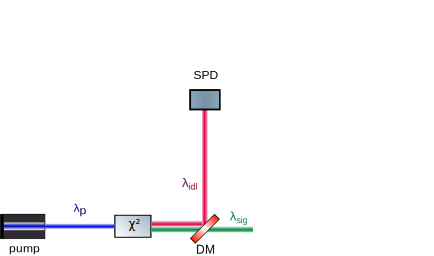
\includegraphics[width=.7\textwidth]{Images/ConventionalSetup_NoSam.pdf}}
			\only<2->{\includegraphics[width=.7\textwidth]{Images/ConventionalSetup.pdf}}
		\end{minipage}%
		\hfill
		\begin{minipage}{0.35\textwidth}
			\[
			\begin{aligned}
				\uncover<1->{N_{\text{sing}}^{\text{ref}} &= \eta_{\text{idl}} N_{\mathrm{g}} + N_{\text{noise}}^{\text{ref}}} \\[0.5em]
				\uncover<2->{N_{\text{sing}}^{\text{sam}} &= T\,\eta_{\text{idl}} N_{\mathrm{g}} + N_{\text{noise}}^{\text{sam}} } \\[1em]
				\uncover<3->{\Rightarrow T &= \frac{\,N_{\text{sing}}^{\text{sam}} - N_{\text{noise}}^{\text{sam}}\,}
				{\,N_{\text{sing}}^{\text{ref}} - N_{\text{noise}}^{\text{ref}}\,} }
			\end{aligned}
			\]
		\end{minipage}
		\visible<4->{
		\begin{center}
			\vspace*{1.5em}
			\resizebox{\textwidth}{!}{$
				\operatorname{Var}(T) 
				= \left( \eta_{\text{idl}}\,N_{\mathrm{g}} \right)^{-2}
				\Bigg[
				\operatorname{Var}\!\left(N_{\text{sing}}^{\text{sam}}\right)
				+ \operatorname{Var}\!\left(N_{\text{noise}}^{\text{sam}}\right) 
				+ T^{2} \Big[ 
				\operatorname{Var}\!\left(N_{\text{sing}}^{\text{ref}}\right) 
				+ \operatorname{Var}\!\left(N_{\text{noise}}^{\text{ref}}\right)
				\Big]
				\Bigg]
				$}
		\end{center}
		}
	\end{frame}
		
	
	\begin{frame}[b]{Coincidence approach}
		\begin{minipage}{.6\textwidth}
			\centering
			\only<1>{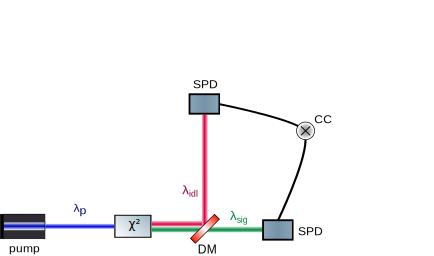
\includegraphics[width=.9\textwidth]{Images/CoincSetup_NoSam.pdf}}
			\only<2->{\includegraphics[width=.9\textwidth]{Images/CoincSetup_Sam.pdf}}
		\end{minipage}
		\hfill
		\begin{minipage}{.35\textwidth}
			\[
			\begin{aligned}
				\uncover<1->{N_{\text{coin}}^{\text{ref}} &= \eta_{\text{idl}} \,\eta_{\text{sig}} \, N_{\mathrm{g}} + N_{\text{ac}}^{\text{ref}} } \\[1em]
				\uncover<2->{N_{\text{coin}}^{\text{sam}} &= T \,\eta_{\text{idl}} \,\eta_{\text{sig}} \, N_{\mathrm{g}} + N_{\text{ac}}^{\text{sam}} } \\[1em]
				\uncover<3->{
				\Rightarrow T &= \frac{\,N_{\text{coin}}^{\text{sam}} - N_{\text{ac}}^{\text{sam}}\,}{\,N_{\text{coin}}^{\text{ref}} - N_{\text{ac}}^{\text{ref}}\,}
				} 
			\end{aligned}
			\]
		\end{minipage}
		\visible<4->{
			\begin{center}
				\vspace*{1.5em}
				\resizebox{\textwidth}{!}{$
					\operatorname{Var}(T) 
					= \left( \eta_{\text{sig}}\,\eta_{\text{idl}}\,N_{\mathrm{g}} \right)^{-2}
					\Bigg[
					\operatorname{Var}\!\left(N_{\text{coin}}^{\text{sam}}\right)
					+ \operatorname{Var}\!\left(N_{\text{ac}}^{\text{sam}}\right) 
					+ T^{2} \Big[ 
					\operatorname{Var}\!\left(N_{\text{coin}}^{\text{ref}}\right)
					+ \operatorname{Var}\!\left(N_{\text{ac}}^{\text{ref}}\right) 
					\Big]
					\Bigg]
					$}
			\end{center}
		}
	\end{frame}
	
%	\begin{aligned}
%		\uncover<1->{N_{\text{cc,pure}}^{\text{ref}} &= \eta_{\text{idl}} \,\eta_{\text{sig}} \, N_{\mathrm{g}} \\[0.5em]
%			N_{\text{cc,tot}}^{\text{ref}} &= N_{\text{cc,pure}}^{\text{ref}} + N_{\text{ac}}^{\text{ref}} } \\[1em]
%		\uncover<2->{N_{\text{cc,pure}}^{\text{sam}} &= T \,\eta_{\text{idl}} \,\eta_{\text{sig}} \, N_{\mathrm{g}} \\[0.5em]
%			N_{\text{cc,tot}}^{\text{sam}} &= N_{\text{cc,pure}}^{\text{sam}} + N_{\text{ac}}^{\text{sam}} } \\[1em]
%		\uncover<3->{
%			\Rightarrow T &= \frac{\,N_{\text{tot,cc}}^{\text{sam}} - N_{\text{ac}}^{\text{sam}}\,}{\,N_{\text{tot,cc}}^{\text{ref}} - N_{\text{ac}}^{\text{ref}}\,}
%		} 
%	\end{aligned}
	
	\begin{frame}{Transmittance model}
		\begin{Block}{Conventional approach:}
			\vspace{0.5em}
			\resizebox{\textwidth}{!}{$
				\operatorname{Var}(T) 
				= \left( \eta_{\text{idl}}\,N_{\mathrm{g}} \right)^{-2}
				\Bigg[
				\textcolor<2->{red}{\operatorname{Var}\!\left(N_{\text{sing}}^{\text{sam}}\right)} 
				+ \textcolor<2->{red}{\operatorname{Var}\!\left(N_{\text{noise}}^{\text{sam}}\right)} 
				+ T^{2} \Big[ 
				\textcolor<2->{red}{\operatorname{Var}\!\left(N_{\text{sing}}^{\text{ref}}\right)} 
				+ \textcolor<2->{red}{\operatorname{Var}\!\left(N_{\text{noise}}^{\text{ref}}\right) }
				\Big]
				\Bigg]
			$}
		\end{Block}
		\vspace*{2em}
		\begin{Block}{Coincidence approach:}
			\vspace{0.5em}
			\resizebox{\textwidth}{!}{$
				\operatorname{Var}(T) 
				= \left( \eta_{\text{sig}}\,\eta_{\text{idl}}\,N_{\mathrm{g}} \right)^{-2}
				\Bigg[
				\textcolor<2>{red}{\operatorname{Var}\!\left(N_{\text{coin}}^{\text{sam}}\right) }
				+ \textcolor<2>{red}{\operatorname{Var}\!\left(N_{\text{ac}}^{\text{sam}}\right) }
				+ T^{2} \Big[ 
				\textcolor<2>{red}{\operatorname{Var}\!\left(N_{\text{coin}}^{\text{ref}}\right) }
				+ \textcolor<2>{red}{\operatorname{Var}\!\left(N_{\text{ac}}^{\text{ref}}\right) }
				\Big]
				\Bigg]
			$}
		\end{Block}
	\end{frame}
%	\begin{frame}{Photon statistics}
%		\begin{minipage}{.3\textwidth}
%			\visible<2->{
%			\begin{tikzpicture}
%				\begin{axis}[
%					width=1.2\linewidth,
%					height=1.4\linewidth,
%					xlabel={$n\,\,[a.u.]$},
%					ylabel={$\mathcal{P}(n)\,\,[a.u.]$},
%					xticklabels={},
%					yticklabels={},
%					%grid=major,
%					scaled y ticks = false,
%					tick label style={font=\small},
%					label style={font=\small},
%					legend style={font=\tiny,
%						draw=none,      
%						fill=none,  },
%					]
%					\only<2->{
%					\addplot [mark=none, color=blue, very thick] 
%					table [x index=0, y index=1, header=false] {Images/photon_distributions.txt};
%					\addlegendentry{Poisson}
%					}
%					
%					\only<3->{
%					\addplot [mark=none, color=black, very thick] 
%					table [x index=0, y index=2, header=false] {Images/photon_distributions.txt};
%					\addlegendentry{mmBE}
%					}
%				\end{axis}
%			\end{tikzpicture}
%			}
%		\end{minipage}
%		\hfill
%		\begin{minipage}{.65\textwidth}
%			\visible<2->{
%			Poisson distribution (coherent light): %\footnote{\fullcite{kimPhotoncountingStatisticsbasedSupport2022,schneelochIntroductionAbsoluteBrightness2019}}
%			\[
%			\begin{aligned}
%				\mathcal{P}(n) &= \frac{\langle n\rangle^{n}}{n!}\,e^{-\langle n\rangle} \\ \vspace{5em}
%				\operatorname{Var}(n) &= \langle n\rangle
%			\end{aligned}
%			\]
%			}
%			\visible<3->{
%			multi-mode Bose-Einstein distribution:
%			\[
%			\begin{aligned}
%				\mathcal{P}_m(n) &= \frac{(n+m-1)!}{(m-1)!\,n!}\,
%				\frac{m^m\langle n\rangle^{n}}{\left(m+\langle n\rangle\right)^{n+m}} \\ \vspace{5em}
%				\operatorname{Var}(n) &= \langle n\rangle \left(1+\frac{\langle n\rangle}{m}\right)
%			\end{aligned}
%			\]
%			}
%		\end{minipage}
%	\end{frame}
	
		\begin{frame}{Photon statistics}

			\visible<2->{
				Poisson distribution (coherent light): \only<3->{\footnote{\authortitlefootcite{kimPhotoncountingStatisticsbasedSupport2022}}\footnote{\authortitlefootcite{foucheDetectionFalsealarmProbabilities2003}} } 
				\[
				\begin{aligned}
					\mathcal{P}(n) &= \frac{\langle n\rangle^{n}}{n!}\,e^{-\langle n\rangle} \\ \vspace{5em}
					\operatorname{Var}(n) &= \langle n\rangle
				\end{aligned}
				\]
			}
			\visible<4->{
				Multi-mode Bose-Einstein distribution (thermal light): \footnotemark[2]
				\[
				\begin{aligned}
					\mathcal{P}_m(n) &= \frac{(n+m-1)!}{(m-1)!\,n!}\,
					\frac{m^m\langle n\rangle^{n}}{\left(m+\langle n\rangle\right)^{n+m}} \\ \vspace{5em}
					\operatorname{Var}(n) &= \langle n\rangle \left(1+\frac{\langle n\rangle}{m}\right)
				\end{aligned}
				\]
			}

	\end{frame}
	
	\section{Experiment}
	\begin{frame}{Experimental setup}
		\begin{minipage}{.5\textwidth}
			\begin{center}
				\includegraphics[width=\textwidth]{Images/DupishSetupNew.pdf}
			\end{center}
		\end{minipage}
		\hfill
		\begin{minipage}{.45\textwidth}
			\begin{tikzpicture}
				
				\visible<2->{
				\node (top) at (0,0) 		{\includegraphics[width=.9\textwidth]{Images/ExampleCountsExp.pdf}};
					}
					
				\visible<3->{
				\node (bottom) at (0,-3.6) 		{\includegraphics[width=.9\textwidth]{Images/ExampleHistoExp.pdf}};
				
				\draw[-{Latex[length=2mm]}, thick]	([xshift=3mm] top.south)
						-- 
						([xshift=3mm] bottom.north);
					}
			\end{tikzpicture}
			\end{minipage}
	\end{frame}
	
	
	\section{Results}
	
	\begin{frame}[b]{Dark counts, $\operatorname{Var}\!\left(N_{\text{noise}}\right)$}
		\visible<2->{
		\begin{minipage}{.45\textwidth}
			\centering
			Signal arm
			%\vspace{2em}
			\includegraphics[width=\textwidth]{Images/DC_Sig_2.pdf}
		\end{minipage}
		}
		\hfill
		\visible<3->{
		\raisebox{-1.8em}{
		\begin{minipage}{.45\textwidth}
			\centering
			Idler arm \\[.2em]
			
			\includegraphics[width=\textwidth]{Images/DC_Idl_2.pdf}
			\visible<4->{
				%\vspace*{1em}
			{\footnotesize
				\[
				\operatorname{Var}\!\left(N_{\text{noise}}\right) = 1.8 \cdot \langle N_{\text{noise}} \rangle
				\]
			}
			}
		
		\end{minipage}
		}
		}
	\end{frame}
	
	\begin{frame}[b]{Single counts, $\operatorname{Var}\!\left(N_{\text{sing}}\right)$}
		\visible<2->{
		\begin{minipage}{.45\textwidth}
			\centering
			Signal arm \\[.3em]
			
			\includegraphics[width=\textwidth]{Images/SingleStatisticsSignal_4.pdf}
		\end{minipage}
		}
		\hfill
		\visible<3->{
			\raisebox{-1.5em}{
		\begin{minipage}{.45\textwidth}
			\centering
			Idler arm \\[.5em]
			%\vspace*{-1em}
			\includegraphics[width=\textwidth]{Images/SingleStatisticsIdler_4.pdf}
			\\[-1em]
			\visible<4->{
			{\footnotesize
				\[
				\operatorname{Var}\!\left(N_{\text{sing}}\right) = 2.2 \cdot \langle N_{\text{sing}} \rangle
				\]
			}
			}
		\end{minipage}
			}
		}
	\end{frame}
	
	\begin{frame}[b]{Coincidence counts, $\operatorname{Var}\!\left(N_{\text{coin}}\right)$}
		\visible<2->{
		\begin{minipage}{.45\textwidth}
			\centering
			Coincidences \\[0.5em]
			\includegraphics[width=\textwidth]{Images/CoincStatistics_2.pdf}
			%\vspace*{-2.5em}
			\visible<3->{
			{\footnotesize
				\[
				\operatorname{Var}\!\left(N_{\text{coin}}\right) = \langle N_{\text{coin}} \rangle
			\]
			}
			}
		\end{minipage}
		}
		\hfill
		\visible<4->{
		\begin{minipage}{.45\textwidth}
			\centering
			Accidentals \\[0.5em]
			\includegraphics[width=\textwidth]{Images/AccCountsStatistics_2.pdf}
			%\vspace*{-2.5em}
			\visible<5->{
				{\footnotesize
					\[
				\operatorname{Var}\!\left(N_{\text{ac}}\right) = \langle N_{\text{ac}} \rangle
			\]
			}
			}
		\end{minipage}
		}
	\end{frame}
	
	
	\section{Simulation}
	\begin{frame}{Simulation}
		\begin{Block}{Conventional approach:}
			\vspace{0.5em}
			\only<1>{
				\resizebox{\textwidth}{!}{$
					\operatorname{Var}(T) 
					= \left( \eta_{\text{idl}}\,N_{\mathrm{g}} \right)^{-2}
					\Bigg[
					\operatorname{Var}\!\left(N_{\text{sing}}^{\text{sam}}\right)
					+ \operatorname{Var}\!\left(N_{\text{noise}}^{\text{sam}}\right)
					+ T^{2}\Big[
					\operatorname{Var}\!\left(N_{\text{sing}}^{\text{ref}}\right)
					+ \operatorname{Var}\!\left(N_{\text{noise}}^{\text{ref}}\right)
					\Big]
					\Bigg]
					$}
			}
			
			% version with <N>
			\only<2->{%
				\resizebox{\textwidth}{!}{$
					\operatorname{Var}(T) 
					= \left( \eta_{\text{idl}}\,N_{\mathrm{g}} \right)^{-2}
					\Bigg[\textcolor{red}{2.2\cdot
					\langle N_{\text{sing}}^{\text{sam}}\rangle}
					+ \textcolor{red}{1.8\cdot\langle N_{\text{noise}}^{\text{sam}}\rangle}
					+ T^{2}\Big[
					\textcolor{red}{2.2\cdot\langle N_{\text{sing}}^{\text{ref}}\rangle}
					+ \textcolor{red}{1.8\cdot\langle N_{\text{noise}}^{\text{ref}}\rangle}
					\Big]
					\Bigg]
					$}
			}
		\end{Block}
		

		\vspace*{2em}
		\visible<3->{
		\begin{Block}{Coincidence approach:}
			\vspace{0.5em}
			\only<3>{
				\resizebox{\textwidth}{!}{$
					\operatorname{Var}(T) 
					= \left( \eta_{\text{sig}}\,\eta_{\text{idl}}\,N_{\mathrm{g}} \right)^{-2}
					\Bigg[
					\operatorname{Var}\!\left(N_{\text{coin}}^{\text{sam}}\right)
					+ \operatorname{Var}\!\left(N_{\text{ac}}^{\text{sam}}\right) 
					+ T^{2} \Big[ 
				\operatorname{Var}\!\left(N_{\text{coin}}^{\text{ref}}\right) 
					+ \operatorname{Var}\!\left(N_{\text{ac}}^{\text{ref}}\right) 
					\Big]
					\Bigg]
					$}
			}
			
			% version with <N>
			\only<4->{%
				\centering
				\resizebox{.8\textwidth}{!}{$
					\operatorname{Var}(T) 
					= \left( \eta_{\text{sig}}\,\eta_{\text{idl}}\,N_{\mathrm{g}} \right)^{-2}
					\Bigg[
					\textcolor{red}{\langle N_{\text{coin}}^{\text{sam}}\rangle }
					+ \textcolor{red}{\langle N_{\text{ac}}^{\text{sam}}\rangle }
					+ T^{2} \Big[ 
					\textcolor{red}{\langle N_{\text{coin}}^{\text{ref}}\rangle }
					+ \textcolor{red}{\langle N_{\text{ac}}^{\text{ref}}\rangle }
					\Big]
					\Bigg]
					$}
			}
		\end{Block}
		}
	\end{frame}
	
	\begin{frame}{Simulation}
		\begin{minipage}{0.45\textwidth}
			% --- TOP IMAGE ---
			\visible<2->{
			\begin{minipage}{0.70\textwidth}
				\includegraphics[width=\textwidth]{Images/SweepSinglesIdler_Eff_70_70_NoNoise.pdf}
			\end{minipage}
			\hfill
			\begin{minipage}{0.25\textwidth}
				\raisebox{2em}{%
				{\tiny
					\(
					\begin{aligned}
						\eta_{\text{idl}} &= \text{70}\% \\
						\eta_{\text{sig}} &= \text{70}\% \\
						R_{\text{noise,idl}} &= \text{0}~\text{Hz}
					\end{aligned}
					\)
				}
			}
			\end{minipage}%
			}
			\vspace{1.5em}
			
			% --- BOTTOM IMAGE ---
			\visible<3->{
			\begin{minipage}{0.70\textwidth}
				\includegraphics[width=\textwidth]{Images/SweepSinglesIdler_Eff_2-6_009_NoNoise.pdf}
			\end{minipage}
			\hfill
			\begin{minipage}{0.25\textwidth}
				\raisebox{2em} \\
						\eta_{\text{sig}} &= \textcolor{red}{\text{2.6}\%} \\
						R_{\text{noise,idl}} &= \text{0}~\text{Hz}
					\end{aligned}
					\)
					}
				}
			\end{minipage}%
			}
		\end{minipage}
		\hfill
		\begin{minipage}{0.5\textwidth}
			
			\visible<4->{
			\begin{minipage}{0.70\textwidth}
				\includegraphics[width=\textwidth]{Images/SweepSinglesIdler_Eff_2-6_009_20kNoise.pdf}
			\end{minipage}
			\hfill
			\begin{minipage}{0.25\textwidth}
				\raisebox{2em}{%
					{\tiny
						\(
					\begin{aligned}
						\eta_{\text{idl}} &= \text{0.09}\% \\
						\eta_{\text{sig}} &= \text{2.6}\% \\
						R_{\text{noise,idl}} &= \textcolor{red}{\text{20 kHz}}
					\end{aligned}
					\)
					}
				}
			\end{minipage}
			}
		\end{minipage}
	\end{frame}
	
	
%		\begin{frame}{Simulation}
%		\begin{minipage}{0.45\textwidth}
%			% --- TOP IMAGE ---
%			\visible<2->{
%					\includegraphics[width=.8\textwidth]{Images/SweepSinglesIdler_Eff_70_70_NoNoise_WLeg.pdf}
%			}
%			\vspace*{1em}
%			
%			% --- BOTTOM IMAGE ---
%			\visible<3->{
%					\includegraphics[width=.8\textwidth]{Images/SweepSinglesIdler_Eff_2-6_009_NoNoise_WLeg.pdf}
%
%			}
%		\end{minipage}
%		\hfill
%		\begin{minipage}{0.5\textwidth}
%			
%			\visible<4->{
%					\includegraphics[width=.9\textwidth]{Images/SweepSinglesIdler_Eff_2-6_009_20kNoise_WLeg.pdf}
%
%			}
%		\end{minipage}
%	\end{frame}
	
	
	\begin{frame}{Noise-to-signal ratio}
		\begin{minipage}{.55\textwidth}
			\centering
			\includegraphics[width=\textwidth]{Images/SimulationSweepSNR_MultEff.pdf}
		\end{minipage}
		\hfill
		\begin{minipage}{.35\textwidth}
			\raisebox{5em}{%
			\resizebox{\linewidth}{!}{%
				\begin{tabular}{@{}l@{\hspace{50pt}}lll@{}}
					\toprule[1.5pt]
					\textbf{Parameter} &  \textbf{Value}\\
					\midrule
					$\eta_{\text{idl}}$ (\%) & 0.09 \\
					$\eta_{\text{sig}}$ (\%) & 2.6, 5, 20 \\
					\textcolor{red}{$R_{\text{idl}}$ (kHz)} & \textcolor{red}{1 - 20} \\
					$R_{\text{noise,idl}}$ (kHz) & 20\\
					$R_{\text{noise,sig}}$ (Hz)  & 7 \\
					$T$ (1) & 0.9\\
					\bottomrule[1.5pt]
				\end{tabular}
			}
			}
		\end{minipage}
	\end{frame}
	
	
%	\begin{frame}{Transmittance}
%		\begin{minipage}{.55\textwidth}
%			\centering
%			\includegraphics[width=\textwidth]{Images/SimulationSweepTrans}
%		\end{minipage}
%		\hfill
%		\begin{minipage}{.35\textwidth}
%			\resizebox{\linewidth}{!}{%
%				\begin{tabular}{@{}l@{\hspace{50pt}}lll@{}}
%					\toprule[1.5pt]
%					\textbf{Parameter} &  \textbf{Value}\\
%					\midrule
%					$\eta_{\text{idl}}$ (\%) & 0.09 \\
%					$\eta_{\text{sig}}$ (\%) & 2.6 \\
%					$R_{\text{idl}}$ (kHz) & 10 \\
%					$R_{\text{noise,idl}}$ (kHz) & 100\\
%					$R_{\text{noise,sig}}$ (Hz)  & 7 \\
%					\textcolor{red}{$T$ (1)} & \textcolor{red}{0 - 1}\\
%					\bottomrule[1.5pt]
%				\end{tabular}
%			}
%		\end{minipage}
%	\end{frame}
	
	\section{Summary}
	
	\begin{frame}{Summary and Outlook}
		\visible<2->{
		\begin{block}{Summary:}
			\begin{itemize}
				\item Established a model for the variance of transmittance
				\item Experimental verification of photon statistics
				\item Found regions where coincidence approach offers higher precision
			\end{itemize}
		\end{block}
		}
		\visible<3->{
		\begin{block}{Outlook:}
			\begin{itemize}
				\item Experimental verification of the found parameter regions
				\item Determine the experimental limiations for the variance measurement
			\end{itemize}
		\end{block}
		}

	\end{frame}
	
	\appendix
	%Appendix
	
	%\backupbegin
	
	\begin{frame}{Accidental counts}
		\begin{minipage}{.5\textwidth}
			\centering
			\includegraphics[width=\textwidth]{Images/AccCountsTheoExpStep4_2}
		\end{minipage}
		\hfill
		\begin{minipage}{.45\textwidth}
			\vspace*{-1em}
			{\small
				\[
				\begin{aligned}
					R_{\text{ac}}^{\text{sam}} 
					&= \Big( T\,\eta_{\text{idl}} R_{\mathrm{g}} + R_{\text{dc,idl}} - R_{\mathrm{cc,pure}}^{\mathrm{sam}} \Big) \cdot \\
					& \hspace*{2.5ex}
					\Big( \eta_{\text{sig}} R_{\mathrm{g}} + R_{\text{dc,sig}} - R_{\text{cc,pure}}^{\text{sam}} \Big) \cdot
					\tau_{\text{cw}} \\[1.5em]
					R_{\text{ac}}^{\text{ref}} 
					&= \Big( \eta_{\text{idl}} R_{\mathrm{g}} + R_{\text{dc,idl}} - R_{\text{cc,pure}}^{\text{ref}} \Big) \cdot \\ & \hspace*{2.5ex}
					\Big( \eta_{\text{sig}} R_{\mathrm{g}} + R_{\text{dc,sig}} - R_{\text{cc,pure}}^{\text{ref}} \Big) \cdot
					\tau_{\text{cw}}
				\end{aligned}
				\]
			}
		\end{minipage}
	\end{frame}
	
	\begin{frame}{Heralding efficiencies}
		\begin{minipage}{.55\textwidth}
			\centering
			\includegraphics[width=\textwidth]{Images/HeraldingEff_2}
		\end{minipage}
		\hfill
		\begin{minipage}{.4\textwidth}
			\vspace*{-2em}
			{\small
			\[
				\begin{aligned}
				\eta_{\text{sig}} &= \frac{N_{\text{coin}}-N_{\text{ac}}}{N_{\text{sing,idl}}-N_{\text{noise}}} = \frac{\eta_{\text{sig}}\eta_{\text{idl}}N_{\text{g}}}{\eta_{\text{idl}}N_{\text{g}}} \\[1em]
				\eta_{\text{idl}} &= \frac{N_{\text{coin}}-N_{\text{ac}}}{N_{\text{sing,sig}}-N_{\text{noise}}} = \frac{\eta_{\text{sig}}\eta_{\text{idl}}N_{\text{g}}}{\eta_{\text{sig}}N_{\text{g}}}
				\end{aligned}
			\]
			}
		\end{minipage}
		
	\end{frame}
	
	\begin{frame}{Histogram}
		\centering
		\includegraphics[width=.7\textwidth]{Images/HistogramExample_2}
	\end{frame}
	
	\begin{frame}{Afterpulsing}
		\begin{minipage}{.6\textwidth}
			\centering
			\includegraphics[width=\textwidth]{Images/VarMean_DeadTime_Afterpulsing_2}
		\end{minipage}
		\hfill
		\begin{minipage}{.35\textwidth}
			{
				\[
					R_{aft} \propto e^{-\frac{t_d}{\tau_{de}}} 
				\]
			}
		\end{minipage}
		\hspace*{-3em}\footnote{\authortitlefootcite{humerSimpleRobustMethod2015}}
	\end{frame}
	
	\begin{frame}{Noiseless case}
		\begin{minipage}{.55\textwidth}
			\centering
			\includegraphics[width=\textwidth]{Images/Appendix_SweepTrans0Noise.pdf}
		\end{minipage}
		\hfill
		\begin{minipage}{.35\textwidth}
			\resizebox{\linewidth}{!}{%
				\begin{tabular}{@{}l@{\hspace{50pt}}lll@{}}
					\toprule[1.5pt]
					\textbf{Parameter} &  \textbf{Value}\\
					\midrule
					$\eta_{\text{idl}}$ (\%) & 60 \\
					$\eta_{\text{sig}}$ (\%) & 20, 60 \\
					$R_{\text{idl}}$ (kHz) & 1 \\
					$R_{\text{noise,idl}}$ (kHz) & 0\\
					$R_{\text{noise,sig}}$ (Hz)  & 7 \\
					\textcolor{red}{$T$ (1)} & \textcolor{red}{0 - 1}\\
					\bottomrule[1.5pt]
				\end{tabular}
			}
		\end{minipage}
	\end{frame}
	\begin{frame}{In presence of noise}
		\begin{minipage}{.55\textwidth}
			\centering
			\includegraphics[width=\textwidth]{Images/Appendix_SweepTransNSR1.pdf}
		\end{minipage}
		\hfill
		\begin{minipage}{.35\textwidth}
			\resizebox{\linewidth}{!}{%
				\begin{tabular}{@{}l@{\hspace{50pt}}lll@{}}
					\toprule[1.5pt]
					\textbf{Parameter} &  \textbf{Value}\\
					\midrule
					$\eta_{\text{idl}}$ (\%) & 60 \\
					$\eta_{\text{sig}}$ (\%) & 10, 20 \\
					$R_{\text{idl}}$ (kHz) & 1 \\
					$R_{\text{noise,idl}}$ (kHz) & 1\\
					$R_{\text{noise,sig}}$ (Hz)  & 7 \\
					\textcolor{red}{$T$ (1)} & \textcolor{red}{0 - 1}\\
					\bottomrule[1.5pt]
				\end{tabular}
			}
		\end{minipage}
	\end{frame}
	
	\begin{frame}{Coherent Illumination, noiseless}
		\begin{minipage}{.55\textwidth}
			\centering
			\includegraphics[width=\textwidth]{Images/Appendix_SweepTrans0Noise_Coh.pdf}
		\end{minipage}
		\hfill
		\begin{minipage}{.35\textwidth}
			\resizebox{\linewidth}{!}{%
				\begin{tabular}{@{}l@{\hspace{50pt}}lll@{}}
					\toprule[1.5pt]
					\textbf{Parameter} &  \textbf{Value}\\
					\midrule
					$\eta_{\text{idl}}$ (\%) & 60 \\
					$\eta_{\text{sig}}$ (\%) & 60, 90 \\
					$R_{\text{idl}}$ (kHz) & 1 \\
					$R_{\text{noise,idl}}$ (kHz) & 0\\
					$R_{\text{noise,sig}}$ (Hz)  & 7 \\
					\textcolor{red}{$T$ (1)} & \textcolor{red}{0 - 1}\\
					\bottomrule[1.5pt]
				\end{tabular}
			}
		\end{minipage}
	\end{frame}
	\begin{frame}{Coherent Illumination, with noise}
		\begin{minipage}{.55\textwidth}
			\centering
			\includegraphics[width=\textwidth]{Images/Appendix_SweepTransNSR1_Coh.pdf}
		\end{minipage}
		\hfill
		\begin{minipage}{.35\textwidth}
			\resizebox{\linewidth}{!}{%
				\begin{tabular}{@{}l@{\hspace{50pt}}lll@{}}
					\toprule[1.5pt]
					\textbf{Parameter} &  \textbf{Value}\\
					\midrule
					$\eta_{\text{idl}}$ (\%) & 60 \\
					$\eta_{\text{sig}}$ (\%) & 40, 60 \\
					$R_{\text{idl}}$ (kHz) & 1 \\
					$R_{\text{noise,idl}}$ (kHz) & 1\\
					$R_{\text{noise,sig}}$ (Hz)  & 7 \\
					\textcolor{red}{$T$ (1)} & \textcolor{red}{0 - 1}\\
					\bottomrule[1.5pt]
				\end{tabular}
			}
		\end{minipage}
	\end{frame}

	%\backupend
\end{document}
 
